\documentclass[11pt]{article}
\usepackage{amsmath,amsthm,amssymb,fancyhdr,enumitem,tikz,tikz-cd,xcolor}
\usepackage[top=1in]{geometry}
\usepackage[colorlinks=true,linkcolor=blue,citecolor=blue,urlcolor=blue]{hyperref}
\usepackage{pgfplots}
\usepackage{tikz}
\usepackage{tkz-fct}
\usetikzlibrary{arrows,matrix,cd,decorations.markings,positioning}
%\addtolength{\textwidth}{1in}

\tikzset{
  singlehead/.style={-{Stealth[length=3mm]}},
  doublehead/.style={
    postaction={decorate,decoration={markings,
      mark=at position 0.60 with {\arrow{Stealth[length=3mm]}},
      mark=at position 0.85 with {\arrow{Stealth[length=3mm]}}
    }}
  }
}

\theoremstyle{definition}
\newtheorem*{definition*}{Definition}
\newtheorem{problem}{}
\newcommand{\bp}{\begin{problem}}
\newcommand{\ep}{\end{problem}\bigskip}
\theoremstyle{theorem}
\newtheorem*{hint*}{Hint}
\newtheorem*{answer}{Answer}

\DeclareMathOperator{\id}{id}
\newcommand{\R}{\mathbb{R}}
\newcommand{\C}{\mathbb{C}}
\newcommand{\Z}{\mathbb{Z}}
\DeclareMathOperator{\fix}{\mathrm{Fix}}

\begin{document}
\pagestyle{fancy}
\fancyfoot[R,C,L]{}
\fancyhead[R]{\large \textbf{Fall 2025}}
\fancyhead[L]{\large \textbf{Topology HW 4}}

\newcommand{\Top}{\mathbf{Top}}
\newcommand{\Set}{\mathbf{Set}}
\newcommand{\N}{\mathbb{N}}

\bp Carefully prove:
\begin{enumerate}[label=(\alph*)]
\item The quotient of $[0,1]$ obtained by identifying $0$ and $1$ is homeomorphic to $S^1$.
\item That the standard model of the torus obtained by identifying opposite sides of a unit square is homeomorphic to $S^1\times S^1$.
\end{enumerate}
\ep

\bp Let $X=[0,1]$.  Let $S\subseteq X$ be any set that is not open and let $\tau$ be any topology on $X$ that contains all the sets that are open in the usual topology together with (at least) the set $S$.  Prove that $X$ with the topology $\tau$ cannot be compact.
\ep

\bp Let $X=\{n, s, e, w\}$ with the topology 
\[ \{\emptyset, \{n\}, \{s\}, \{n,s\}, \{n, s,e \}, \{n,s,w\}, \{n,s,e,w\}\} \]
Here is a picture:
\[
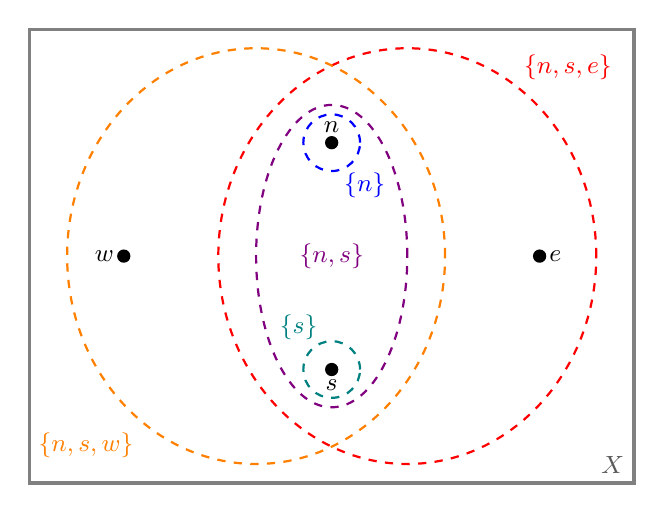
\begin{tikzpicture}[scale=1.2, every node/.style={font=\small}]
  % Points
  \coordinate (N) at (0,1.2);
  \coordinate (S) at (0,-1.2);
  \coordinate (E) at (2.2,0);
  \coordinate (W) at (-2.2,0);

  % Draw points
  \fill (N) circle (2pt) node[above] {$n$};
  \fill (S) circle (2pt) node[below] {$s$};
  \fill (E) circle (2pt) node[right] {$e$};
  \fill (W) circle (2pt) node[left] {$w$};

  % OVALS for open sets (use distinct styles)
  % {n}
  \draw[thick, blue, dashed]
   ($(N)$) ellipse (0.3 and .3);
  \node[blue] at ($(N)+(0.35,-0.45)$) {$\{n\}$};

  % {s}
  \draw[rounded corners=10, thick, dashed, teal]
    ($(S)$) ellipse (0.3 and .3);
  \node[teal] at ($(S)+(-0.35,0.45)$) {$\{s\}$};

  % {n,s}
  \draw[thick, dashed, violet] ($(0,0)$) ellipse (0.8 and 1.6);
  \node[violet] at (0,0) {$\{n,s\}$};

  % {n,s,e}
  \draw[thick, dashed,red] (0.8,0) ellipse (2 and 2.2);
  \node[red] at (2.5,2) {$\{n,s,e\}$};

  % {n,s,w}
  \draw[thick, dashed,orange] (-0.8,0) ellipse (2 and 2.2);
  \node[orange] at (-2.6,-2) {$\{n,s,w\}$};

  % Whole space {n,s,e,w}
  \draw[very thick, gray] (-3.2,-2.4) rectangle (3.2,2.4);
  \node[gray!70!black, anchor=south east] at (3.2,-2.4) {$X$};
\end{tikzpicture}
\]
Even though $X$ only has four points, there are interesting paths in $X$.  For example, $\alpha:[0,1]\to X$ defined by 
\[\alpha(t)=
\begin{cases}
w & \text{ if }0\leq t \leq \frac{1}{3}\\
n & \text{ if }\frac{1}{3}<t<\frac{2}{3}\\
e & \text{ if }\frac{2}{3} \leq t \leq 1.\\
\end{cases}
\]
is a path from $w$ to $e$.
\begin{enumerate}[label=(\alph*)]
\item Is $X$ path connected?
\item Is the map $X \to S^1$ defined by \[w\mapsto (-1,0)\quad n\mapsto (0,1) \quad e \mapsto (1,0) \quad s \mapsto (0,-1)\] continuous?
\item Can you define a map $S^1 \to X$ that is not constant?
\end{enumerate}
\ep



\bp According to \href{https://en.wikipedia.org/wiki/Expansive_homeomorphism}{The Wikipedia article on Expansive Homeomorphism}:
\begin{definition*}
If $( X , d )$ is a metric space, a homeomorphism $f : X \to X$ is said to be expansive if there is a constant $\epsilon >0$, called the \emph{expansivity constant}, such that for every pair of points $x \neq y$ in $X$ there is an integer $n\in \mathbb{Z}$ such that
\[d ( f^n ( x ) , f^n ( y ) ) \geq \epsilon.\]
\end{definition*}

\noindent Note that in this definition, $n$ can be positive or negative.   The Wikipedia article goes on to say \emph{``The space $X$ is often assumed to be compact, since under that assumption expansivity is a topological property.''}  Let's make this remark perfectly clear.

\begin{enumerate}[label=(\alph*)]
\item Show that the two metrics on $\R$ defined by $d_1(x,y)=|x-y|$ and $d_2(x,y)=|e^x-e^y|$ are both compatible with the ordinary topology on $\R$, but the map $f:\R \to \R$ defined by $f(x)=x+1$ is expansive for $d_2$ and not expansive for $d_1$.
\item Suppose $(X,d)$ is a compact.  Prove that if a homeomorphism $f:X \to X$ is expansive for one metric compatible with the topology on $X$ then it is expansive for every metric compatible with the topology on $X$.
\end{enumerate}
\ep

\bp Prove or disprove:
\begin{enumerate}[label=(\alph*)] 
    \item Hausdorff is a homotopy invariant.
    \item Compact is a homotopy invariant.
    \item Path connected is a homotpy invariant.
\end{enumerate}
\ep

\bp Suppose $X$ is Hausdorff and $f:X \to X$.  Prove that the set $\fix(f)=\{x\in X:f(x)=x\}$ is closed.
\ep

\end{document}